  
  This chapter introduces the datasets used for this thesis. Several approaches
  and datasets were considered for evaluating the success of graph machine
  learning on semi-synthetic graphs. In particular, three datasets are 
  considered with varying degrees of success which are:

  \begin{enumerate}
    \item Self launched survey
    \item Bank Telemarketing dataset
    \item US Airline Passenger dataset
  \end{enumerate}

  \noindent The datasets are introduced to the extent that they are successful 
  or useful within the framework of this thesis. In particular, the self 
  launched survey and the Bank Telemarketing dataset showed to be problematic 
  for different reasons. They however provide valuable insights as to when 
  graph machine learning can be successful. These two datasets are therefore 
  only briefly introduced with the focus lying on providing the relevant 
  insights gained from these "failed" datasets. The detailed introduction and
  analysis of these datasets is therefore skipped. The data and the analyses of
  these two datasets are provided in the GitHub repository referenced in
  section \ref{section:software}. The airline passenger satisfaction dataset 
  will be presented in detail, as good results are achieved using graph machine 
  learning. This dataset will also be used for comparing graph machine learning 
  to the standard machine learning models. \\

  \noindent Before introducing the datasets, the programming language and the
   packages used for the analyses are thankfully referenced in the following 
   section. In additon, the GitHub repository containing the datasets and code
   is referenced.

  \section{Software \& Code}
  \label{section:software}

  The entire master's thesis was evaluated using the Python 3.8.10 programming
  language \citep{vanRossum2009}. In addition, following open-source python
  packages were thankfully used which are Numpy 1.20.2 \citep{harris2020array},
  Matplotlib 3.3.4 \citep{Hunter2007}, NetworkX 2.5.1 \citep{hagberg2008exploring}, 
  Seaborn 0.11.1 \citep{Waskom2021}, Pandas 1.2.5 \citep{mckinney2010data}, 
  Statsmodels 0.12.2 \citep{seabold2010statsmodels}, Scikit-Learn 0.24.2 
  \citep{pedregosa2011scikit}, Tensorflow 2.4.0 \citep{abadi2016tensorflow}, 
  Pytorch 1.7.0 \citep{paszke2019pytorch}, deep graph library (dgl) 0.6.1 
  \citep{wang2019deep}, tqdm 4.61.1 \citep{da2021tqdm} and Node2Vec 0.4.3 
  \citep{Cohen2021}. \\

  \noindent The data sets as well as the Python code used for creating and 
  analyzing the data can be found in a public GitHub repository\footnote{GitHub
  repository: \url{https://github.com/MichaelvonSiebenthal/MasterThesis.git}}. 
  The Github repository also includes the Python code for the results shown in
  chapter \ref{section:results}. The GitHub repository serves as a general 
  reference for the data and Python code used for this thesis and will not be 
  referenced individually for every analysis and/or result presented. The GitHub 
  repository includes a read me file which describes which files can be 
  found in which folders. In addition, the Python Code is written in 
  Jupyter Notebooks which include descriptions of the used codes using markdown.

  \section{Self Launched Survey}
  \label{section:self_survey} 

  Initially, the aim was to make use of a self-launched survey which focused on
  a bank client classification task. The classification task was two-fold in 
  that a simpler task focused on classifying bank clients as to whether they 
  would be interested in investing or not. The second classification task
  involved classifying clients according to their investment preferences in
  terms of products (single securities like stocks or bonds, funds, ETFs,
  unsure). The variables used for the graph creation using the MAG model
  included mostly demographic data. Additional data was collected by assessing
  the financial knowledge and behavioral profile of the survey participants by 
  using questions from the financial literacy report of the OECD
  (\citeyear{OECD2017}). The idea was, that demographic data coupled with the 
  financial literacy questions should provide a suitable database for the bank 
  client classification task. \\

  \noindent Unfortunately, only $n=113$ people participated in the survey which 
  in general is very small for a machine learning task.
  Further, the graphs generated using the MAG method were not stable. Due to
  the stochastic element present in the MAG model, the resulting graphs could
  differ dramatically. This lead to significant performance differences for the
  different machine learning methods applied to the resulting graphs.
  Classification accuracies ranged between 40 - 95 \%. A remedy for this 
  problem could be to assign a fixed probability threshold such as 0.5 in the 
  MAG model. Using a fixed threshold probability, the MAG model would 
  generate deterministic graphs, which are always the same. The downside however 
  is, that this makes the graph generation process less realistic. In a
  homophily setting this would assume that a connection is formed with any node 
  where $P[u,v]>0.5$. It is unclear without testing, what impact this would
  have on the graph generation and whether it is positive or negative. It is
  well understood, that people often form connections with people that appear
  unlikely from a probabilistic perspective. This consideration would warrant
  the generation of stochastic graphs. The main priority is however to create
  graphs which provide additional information that can be exploited via graph
  machine learning. Having this objective in mind, it warrants further
  investigation for which the results will be presented in section 
  \ref{section:stoch_det}. \\

  \noindent The self-launched survey could not be used for any meaningful
  analysis due to the small sample size. Nevertheless, it provided an
  interesting follow-up question regarding the question of generating
  stochastic- versus deterministic graphs. The dataset was discarded for
  further analysis and the survey data as well as the performed analyses can be
  found in the GitHub repository. 

  \section{Bank Telemarketing Dataset}
  \label{section:bank_data}

  The Bank Telemarketing dataset first introduced by 
  \cite{moro2011using,moro2014data} was considered as a banking related back-up 
  dataset for the case that the self made survey did not yield a sufficient 
  number of responses. The Bank Relemarketing dataset is based on a marketing 
  campaign at a Portuguese bank. The dataset includes demographic data, data 
  regarding the bank client's wealth, contact success during previous campaigns
  among others. The dataset further provides label data which indicates whether 
  a client invested in a short-term deposit after having been contacted by the
  callcenter of the bank. The dataset is therefore set-up for a binary 
  classification task. The MAG graph generated from the Bank Telemarketing 
  dataset is shown in figure \ref{fig:Moro}.
 
	\begin{figure}[h]
		\centering
		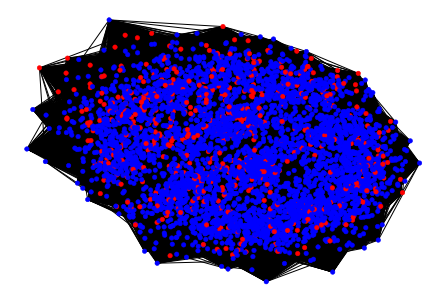
\includegraphics[width=0.7\textwidth]{Moro_network.png}
		\caption{MAG graph of bank telemarketing dataset}
        \label{fig:Moro}
	\end{figure}
  
  \noindent The red dots in figure \ref{fig:Moro} mark the clients which
  decided to invest in the short-term deposit and the blue dots did not invest.
  This figure masks some of the blue nodes due to the figure generation
  process. The general pattern however is apparent. The red nodes are randomly 
  placed in the network which suggests, that graph machine learning will be of
  limited use. The graph further shows, that only a relatively small number of 
  clients appear to have invested in the short-term deposit. To be more precise, 
  only approximately 12\% of bank clients invested in the short-term deposit. 
  The dataset is unbalanced which makes the classification task difficult. Graph 
  representation learning using Node2Vec did not provide any useful results and 
  the GNNs also performed rather poorly. In particular, GNNs tended to classify 
  most clients as non-investors and struggled to accurately classify clients 
  which did invest. Due to the unbalanced data, it is loss optimizing for the
  GNN to predict most nodes as non-investors rather than learning the true
  label. Table \ref{table:Moro_conf} shows the confusion matrix of the 
  classification results for the validation dataset (20\%) using GraphSage.

  \begin{table}[h]
    \centering
    \begin{tabular}{|l|l|c|c}
      \hline
      \diagbox{\textbf{Label}}{\textbf{Predicted}} & \textbf{Did not invest} &
      \textbf{Invested} \\
      \hline
      \textbf{Did not invest} & 1'026 & 30 \\\hline 
      \textbf{Invested} & 119 & 33 \\
      \hline
    \end{tabular}
    \caption{Confusion Matrix Validation Bank Telemarketing Data}
    \label{table:Moro_conf}
  \end{table}

  \noindent The resulting confusion matrix corresponds to an accuracy of
  approximately 87.67\%. The MAG generation process was repeated multiple times
  for which the GraphSage accuracies ranged between 87 - 90\%. Similar results
  were observed for both graph based methods and standard machine learning 
  methods such as ANNs or support vector machines (SVM). \\

  \noindent Unbalanced datasets are part of a larger and common problem in 
  machine learning. Possible remedies might include using loss functions which 
  penalize false classifications harsher than the standard cross entropy loss 
  function used for the GNNs. Alternatively, one could also reduce the data set 
  by dropping observations such that the remaining dataset is balanced. This 
  approach has its own problems as dropping a large number of observations 
  discards a lot of potentially valuable information. It could also put in 
  question the external validity of the model. These comments point to a 
  separate field of research and could be interesting for a future project. \\

  \noindent The failure using graph machine learning methods for this dataset
  reveals, that GNNs are not an easy remedy for unbalanced data. Perhaps, if the
  network structure provided clusters which corresponded to the labels, GNNs
  could provide superior results. Given the variables available in the dataset
  and the limitations of using the MAG method, this was not possible. In order
  to check, whether network structure could indeed remedy the unbalanced label
  problem, the label of the bank telemarketing dataset was used as an
  additional attribute for the MAG model. The label is normally not included as 
  an attribute for the MAG model, as the label data is usually unknown outside 
  of the training dataset. The link-affinity probabilities for the label was set
  as follows:

  \[ \Theta_{label} = 
	\begin{pmatrix}
        0.95 & 0.25 \\
		0.25 & 0.95 \\
	\end{pmatrix}
	\] 
  
  \noindent The resulting MAG graph when considering the label as an attribute 
  is shown in figure \ref{fig:Moro_bias}.

  \begin{figure}[h]
		\centering
		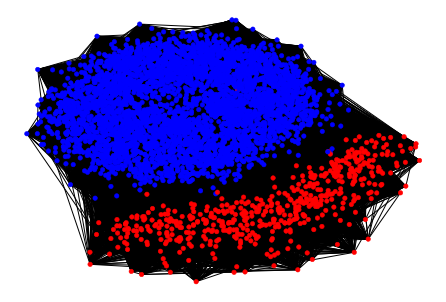
\includegraphics[width=0.7\textwidth]{Moro_network_bias.png}
		\caption{Biased MAG graph of bank telemarketing dataset}
        \label{fig:Moro_bias}
  \end{figure}

  \noindent The nodes shown in figure \ref{fig:Moro_bias} are now nicely
  clustered according to their label. The GNN method GraphSage achieved an 
  accuracy of over 95\% for this graph using otherwise identical feature data
  and model specifications as before. This is of course a form of cheating, as 
  we cannot assume to know the labels of the graph outside of the training 
  setting. In a real-world application, the model would be trained using label
  data and then applied to new data which does not contain the label. We would
  however require the label for the graph generation procedure which makes this
  not a viable approach. Nevertheless, this result shows extremely well when
  graph machine learning can yield superior results compared to standard
  machine learning methods. The key lies in generating a graph with a network
  structure that corresponds to the label. The network structure need not
  necessarily be as clearly separated as shown in figure \ref{fig:Moro_bias}. A
  graph which contains local neighborhood clusters which correspond to the same
  label could yield similar good results. In such a setting, one would have to be
  careful when defining the number of $K$ layers and neighborhood sampling 
  function $\mathcal{N}_{k}$. A network structure which corresponds to
  the label could perhaps also be generated without the label to an extent. This 
  would require the attribute data used in the MAG model to be related with the
  label. The attributes would have to be substitutes for generating a network
  structure which correspond to the label. Given the available attributes for
  the bank telemarketing dataset, this is a difficult task. All features in the 
  dataset have very low correlations with the label. The largest correlation, 
  which is a strong outlier, with the label is call duration with a correlation 
  coefficient $\approx$ 0.3. This value is rather small and a simulation showed, 
  that it could not be used as a single substitute for the label. Selecting the
  appropriate attributes and defining the link-affinity probabilities is not a
  trivial task and requires a lot of trial and error. Unfortunately, for this
  dataset no appropriate attributes and link-affinities were found that yielded
  the desired result. For that reason, this dataset was also discarded. The
  dataset and the performed analyses can be found in the GitHub repository. 

  \section{US Airline Passenger Dataset}
  \label{section:airline_data}

  The US Airline Passenger dataset is a survey which was conducted in 2015
  by J.D. Power \citeyearpar{JDPower2015}. The dataset was retrieved on the 
  website Kaggle \citeyearpar{KAGGLE2015}. This dataset is well suited for 
  applying graph machine learning tasks following the MAG method. It further shows
  to be a competitive dataset for classic machine learning methods. This makes
  this dataset a suitable candidate for a fair comparison of graph machine 
  learning vs standard machine learning. This dataset is presented in detail as 
  it is used for the results presented in chapter \ref{section:results}. \\

  \noindent An overview of the US Airline Passenger dataset is shown in table
  \ref{table:airline_summary}. The correlation heatmap of the dataset is
  further shown in figure \ref{fig:corr_heatmap}. The correlation heatmap
  revealed, that the variables "Departure Delay in Minutes" and "Arrival Delay
  in Minutes" are highly correlated. As "Arrival Delay in Minutes" has some
  missing observations, this variable is dropped in favor of "Departure Delay 
  in Minutes". The heatmap and its corresponding correlation matrix reveal,
  that "Gender" is approximately uncorrelated with any of the other variables.
  Further, "Departure Delay in Minutes" appears to be approximately 
  uncorrelated with any of the other variables. For that reason, it was tested
  whether both variables could be excluded. The results however revealed, that
  the machine learning models performed better if these variables are included 
  in the model. The data shown in table \ref{table:airline_summary} and 
  figure \ref{fig:corr_heatmap} corresponds to a random sample of 6’000 
  observations from the training dataset consisting of 103’904 observations.
  The training graph is created using this sample of 6'000 observations due
  to computational time considerations. 

  \begin{figure}[h]
	  \centering
	  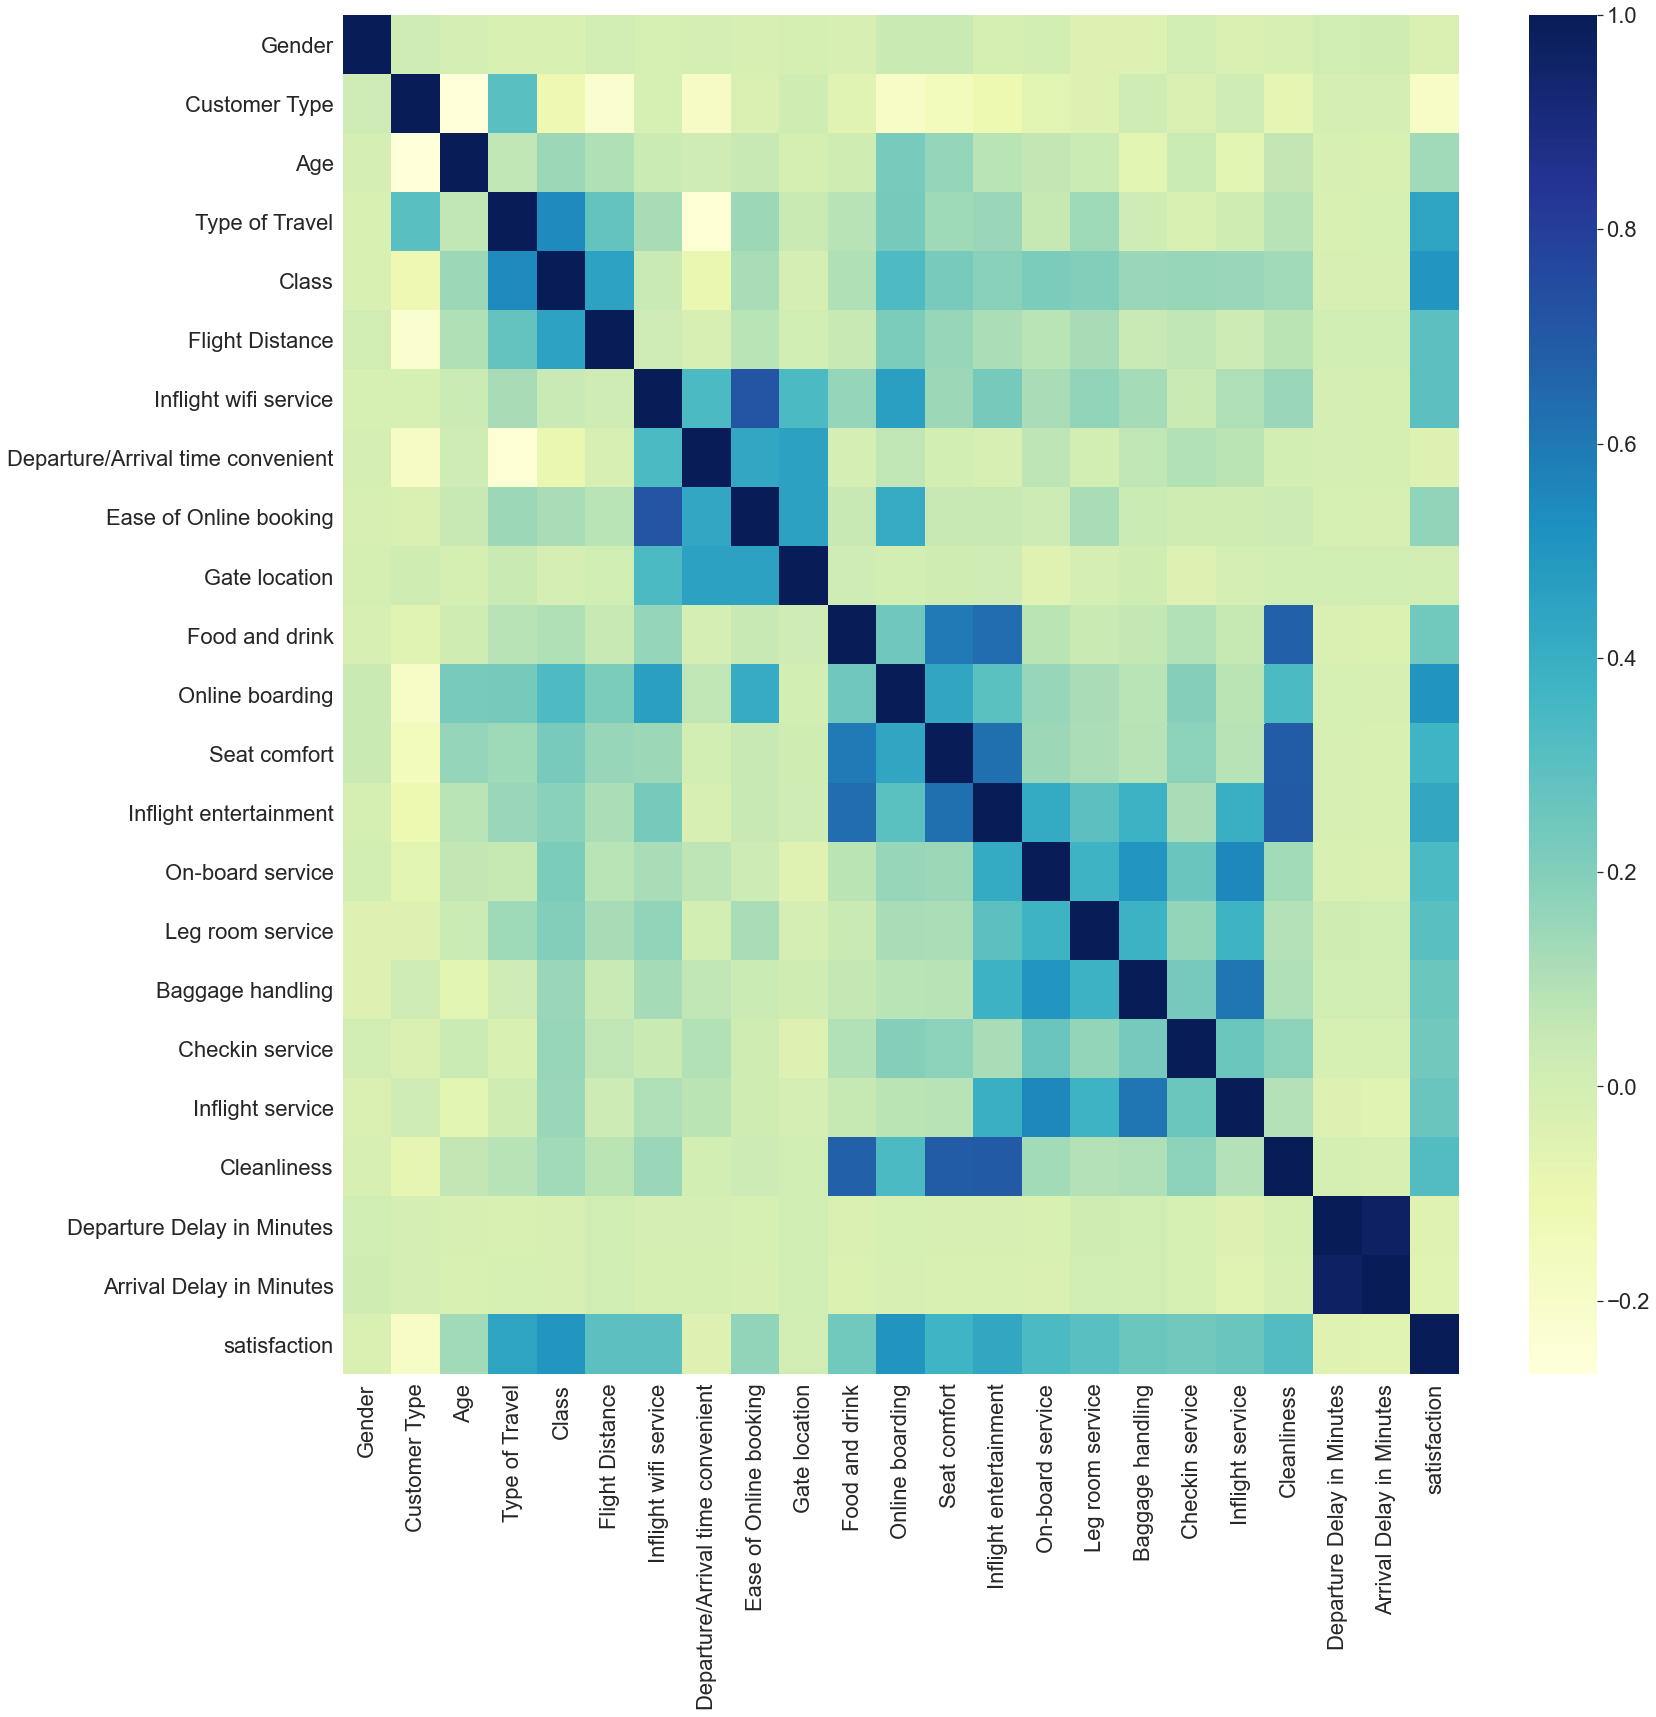
\includegraphics[width=1.0\textwidth]{corr_heatmap.png}
	  \caption{Correlation Heatmap of US Airline Passenger Dataset}
      \label{fig:corr_heatmap}
  \end{figure}

  \begin{landscape}
  \pagestyle{empty}
  \begin{table}[h]
    \centering
    \begin{tabular}{|l|L|c|c|}
      \hline
      \textbf{Variable} & \textbf{Description} & \textbf{Mean} & \textbf{Range} \\
      \hline
      Gender & Gender of the passengers (Male:0, Female:1) & 0.5076 & 0 - 1
      \\\hline 
      Customer Type & The customer type (loyal customer:0, disloyal customer:1) 
      & 0.18 & 0 - 1 \\\hline
      Age & The actual age of the passengers & 39.101 & 7 - 85 \\\hline
      Type of Travel & Purpose of the flight of the passengers
      (Personal Travel:0, Business Travel:1) & 0.6891 & 0 - 1 \\\hline
      Flight Distance & The flight distance of this journey &
      1'197.438 & 67 - 4'963 \\\hline
      Departure Delay in Minutes & Minutes delayed when departure & 14.808 & 0 - 595 \\\hline
      Arrival Delay in Minutes & Minutes delayed when arrival & 15.159 & 0 -
      589 \\\hline
      Satisfied & Satisfaction: Airline satisfaction level(Satisfied, 
      Neutral or Dissatisfaction) & 0.4295 & 0 - 1 \\\hline
      Class & Travel class in the plane of the passengers (Eco:1, Eco Plus:2, 
      Business:3) & - & 1 - 3 \\\hline
      Inflight WiFi service & Satisfaction level of the inflight WiFi service
      (0:Not Applicable;1-5) & - & 0 - 5 \\\hline
      Ease of Online booking & Satisfaction level of online booking & - & 0 - 5
      \\\hline
      Gate location & Satisfaction level of gate location & - & 0 - 5 \\\hline
      Food and drink & Satisfaction level of Food and drink & - & 0 - 5
      \\\hline
      Online boarding & Satisfaction level of online boarding & - & 0 - 5
      \\\hline
      Seat comfort & Satisfaction level of seat comfort & - & 0 - 5 \\\hline
      Inflight entertainment & Satisfaction level of inflight entertainment & -
                             & 0 - 5 \\\hline
      On-board service & Satisfaction level of on-board service & - & 0 - 5
      \\\hline
      Leg room service & Satisfaction level of leg room service & - & 0 - 5
      \\\hline
      Baggage handling & Satisfaction level of baggage handling & - & 0 - 5
      \\\hline
      Check-in service & Satisfaction level of check-in service & - & 0 - 5
      \\\hline
      Inflight service & Satisfaction level of inflight service & - & 0 - 5
      \\\hline
      Cleanliness & Satisfaction level of cleanliness & - & 0 - 5 \\
      \hline
    \end{tabular}
    \caption{Airline Dataset Overview}
    \label{table:airline_summary}
  \end{table}
  \end{landscape}

  \noindent The variables of the dataset are categorized as follows:

  \begin{itemize}
    \item \textbf{Categorical Variables:} Gender, Customer Type, Type of 
      Travel, Satisfaction
    \item \textbf{Ordinal Variables:} Class, Inflight WiFi Service, Ease of Online
      Booking, Gate Location, Food and Drink, Online Boarding, Seat Comfort,
      Inflight Entertainment, On-Board Service, Leg Room Service, Baggage
      Handling, Check-in Service, Inflight Service, Cleanliness
    \item \textbf{Numerical Variables:} Age, Flight Distance, Departure Delay in
      Minutes
  \end{itemize}

  \noindent The categorical variables are dummy coded and the ordinal variable
  Class is coded as shown in table \ref{table:airline_summary}. The remaining 
  ordinal variables which measure different satisfaction levels are recorded 
  using a Likert scale ranging from $1 - 5$. Many passengers did not answer all 
  satisfaction level questions. These responses are recorded with a 0. Therefore, 
  the range of values for the satisfaction level variables range from $0 - 5$. 
  This encoding works well, as a 0 input in a linear pass function of a (graph) 
  neural network will result in a 0 output value. This type of encoding allows 
  for dealing with missing values for neural networks and other machine learning 
  methods. Lastly, the numerical variables had to be normalized. The popular 
  approach of standardizing the entire dataset was unfortunately not possible.
  Due to the missing values prevalent in the satisfaction level variables, it
  must be ensured, that a 0 refers to as a missing response. Note, that a
  recorded 0 for the numerical variables does not correspond to a missing value. 
  The normalizing function applied is defined as follows:

  \begin{equation}
    x' = a + \frac{(x - \min(x))(b - a)}{\max(x) - \min(x)}
    \label{eq:norm}
  \end{equation}

  \noindent In equation \ref{eq:norm}, $x$ refers to the unnormalized 
  variable and $x'$ refers to resulting normalized variable. $a$ defines 
  the lower bound of the normalization range and $b$ is the upper bound. The
  numerical variables are normalized to be within the range 1-5. Now, all 
  variables are within a similar range and different scaling should no longer 
  lead to biasing behavior. \\

  \noindent In the following section, the graph generation process for the US
  Airline Passenger dataset is described in detail.

  \subsection{Graph Generation}
  \label{section:graph_gen}

  To create a graph from the US Airline Passenger dataset, appropriate
  attributes must be selected for the MAG model. The selected attributes must be
  of the type such that realistic probabilities can be assigned. As an example, 
  it is difficult to assign link-affinity probabilities for people who gave 
  ratings regarding the "inflight wifi service". In this case one could assign 
  a probability that people who gave high ratings are more similar with 
  relative ease. However, does this then also translate to people not liking 
  the wifi-service being similar as well? Further, how do we assign 
  probabilities for people who are dissimilar? These considerations make the 
  selection of appropriate attributes difficult. It is therefore important to 
  select attributes for which realistic variables for all of the following
  three settings can be assigned:

  \begin{itemize}
    \item \textbf{Positive similar observations} (e.g. both observations like 
      the service)
    \item \textbf{Negative similar observations} (e.g. both observations 
      dislike the service)
    \item \textbf{Dissimilar observations} (Symmetric for undirected graphs, 
      can be asymmetric for directed graphs)
  \end{itemize}
 
  \noindent The attributes are selected using the above mentioned considerations. 
  The selected attributes with the corresponding link-affinity probabilities are 
  shown in table \ref{table:link_aff}.

  \begin{table}[h]
    \centering
    \begin{tabular}{|l||L|}
      \hline
      \textbf{Attribute Name} & \textbf{Link-Affinity Probabilities}\\
      \hline\hline
      Gender & 0.6, 0.4; 0.4, 0.6  \\\hline 
      Customer Type & 0.8, 0.5; 0.5, 0.8 \\\hline
      Age & 0.90, 0.80, 0.60, 0,40; 0.80, 0.90, 0.80, 0.60; 0.60, 0.80, 0.90,
      0.80; 0.40, 0.60, 0.80, 0.90 \\\hline
      Type of Travel & 0.80, 0.20; 0.20, 0.80 \\\hline
      Class & 0.85, 0.60, 0.45; 0.60, 0.85, 0.60; 0.45, 0.60, 0.85 \\
      \hline
    \end{tabular}
    \caption{Link-Affinity Matrices}
    \label{table:link_aff}
  \end{table}

  \noindent The probabilities in table \ref{table:link_aff} correspond to the
  rows of the link-affinity matrices up to the semi-colon. To give a better
  overview, the link-affinity matrix for age is shown explicitly as follows:

  \[ \Theta_{Age} = 
	\begin{pmatrix}
		0.90 & 0.80 & 0.60 & 0.40 \\
        0.80 & 0.90 & 0.80 & 0.60 \\
        0.60 & 0.80 & 0.90 & 0.80 \\
        0.40 & 0.60 & 0.80 & 0.90 \\
	\end{pmatrix}
  \] 

  \noindent Age is not only selected as an example as it is the largest
  link-affinity matrix. It also requires some additional data transformation.
  It is difficult to use attributes with large cardinalities for the MAG model.
  For that reason, age is binned into 4 categories with 0 if age $<$ 
  26, 1 if 26 $\leqslant$ age $<$ 39, 2 if 39 $\leqslant$ age $<$ 50 and 3 if age
  $\geqslant$ 50. These bins are chosen according to the interquartile lengths 
  present in the distribution of the variable age. \\

  \noindent There exist no clear rules for assigning link-affinity
  probabilities. \citeauthor{kim2012multiplicative} 
  \citeyearpar[p. 118]{kim2012multiplicative} presented the 4 common 
  link-affinity matrix structures of homophily, heterophily, core-periphery and 
  random for creating graphs. Given the selected attribute data, the homophily 
  setting is most appropriate for all link-affinity matrices. In this setting, 
  observations which are similar have a higher probability of forming a 
  connection compared to dissimilar observations. The probabilities are 
  assigned based on personal intuition and trial and error. Several graphs were 
  created using different probabilities, where the probabilities shown in table 
  \ref{table:link_aff} generate the best graphs. There is however no exact 
  science or selection criteria which can be applied for selecting attributes 
  and defining the link-affinity probabilities. \\

  \noindent As mentioned in the previous section, a sub-sample of 6'000 
  observations was retrieved from the training dataset consisting of 103’904 
  observations. With this random sub-sample and the attributes shown in table
  \ref{table:link_aff}, the adjacency matrix for the 
  resulting graph $G(V,E)$ is generated using algorithm \ref{algo:MAG}. The 
  random sub-sample is retrieved due to the computational cost of running 
  algorithm \ref{algo:MAG}. Simulations which involved creating graphs with 
  different random sub-samples show, that the random sub-samples are 
  representative for the entire dataset. This is further supported when 
  comparing the summary statistics of the sub-samples with the full-dataset. 
  The generated graph is shown in figure \ref{fig:us_airline_graph}.

  \begin{figure}[h]
	  \centering
	  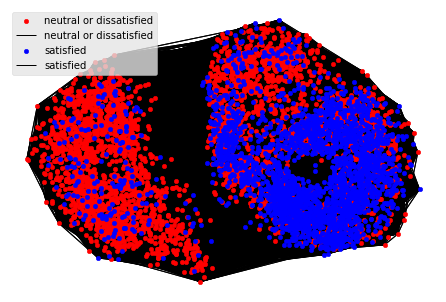
\includegraphics[width=0.7\textwidth]{us_airline_graph.png}
	  \caption{Graph of US Airline Passenger Dataset}
      \label{fig:us_airline_graph}
  \end{figure}
  
  \noindent The network in figure \ref{fig:us_airline_graph} shows the 
  emergence of two primary clusters. In addition one can see, that most satisfied 
  airline passengers appear to be grouped together in the right cluster. To 
  gain a deeper understanding of the dynamics involved in the network formation, 
  the nodes of the network are plotted excluding the edges in figure
  \ref{fig:us_airline_nodes}.

  \begin{figure}[h]
	  \centering
	  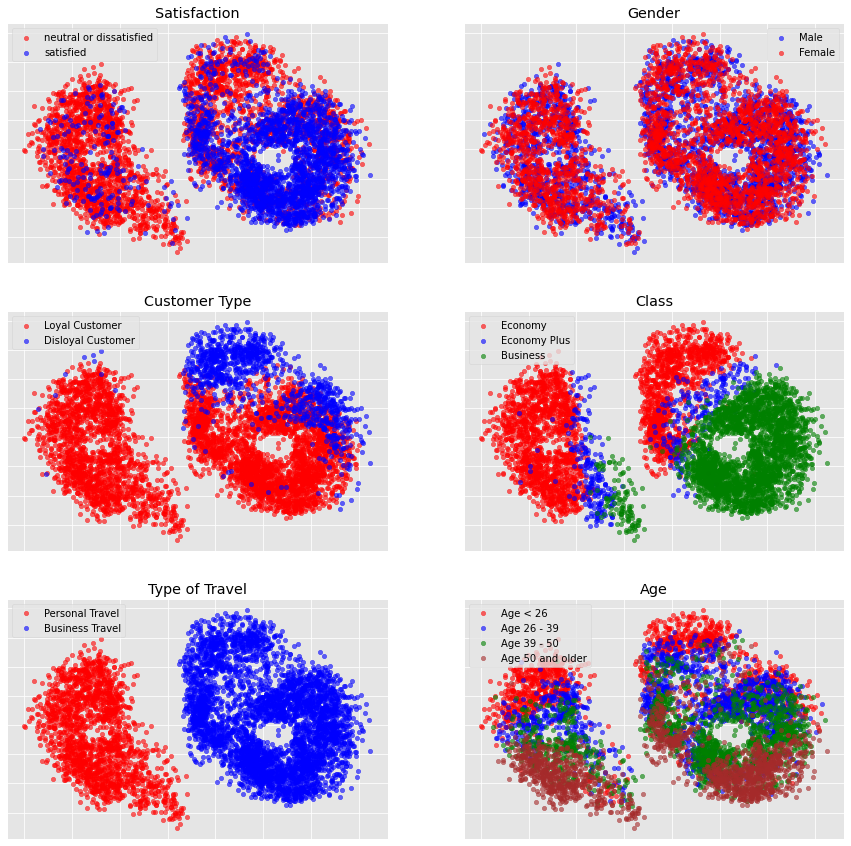
\includegraphics[width=0.8\textwidth]{us_airline_nodes.png}
	  \caption{Graph Nodes of US Airline Passenger Dataset}
      \label{fig:us_airline_nodes}
  \end{figure}

  \noindent Figure \ref{fig:us_airline_nodes} plots the nodes of the network
  for the label "Satisfaction" and the 5 attributes used for the graph
  generation. The transparency of the plot was set to $\alpha = 0.6$ to avoid 
  covering nodes during the graph plotting process. Figure
  \ref{fig:us_airline_nodes} reveals interesting associations. First it is
  shown, that a larger number of people traveling for business purposes are 
  satisfied compared to people traveling for personal reasons. This association
  becomes clear when comparing the Satisfaction plot with the Type of Travel
  plot. In relative terms, only approximately 9.8\% of passengers traveling for 
  personal reasons were satisfied compared to business travelers with a 57.8\% 
  satisfaction rate. Interestingly, passengers traveling for business purposes
  adhere somewhat expected characteristics such as:

  \begin{enumerate}
    \item Most business class passengers are satisfied. 
    \item Older passengers appear to be more satisfied which is largely
      associated with booking more business class tickets. The age plot however 
      reveals, that older passengers tend to be mostly satisfied even when 
      booking economy class.
    \item Most loyal customers book business class. There is some overlap where 
      loyal customers also book economy class tickets. The reverse is true as 
      well, where a cluster of disloyal customers book business class. 
  \end{enumerate}
  
  \noindent Passengers traveling for personal reasons do not appear to adhere
  to the characteristics or associations shown for business travelers. The only
  distinctive character is, that almost all passenger traveling for personal
  reasons are loyal customers. This fact does however not appear to be
  associated with satisfaction. At first, this seems like a rather bizarre 
  finding. Upon further reflection, this could point to a sampling bias of 
  passengers traveling for personal reasons due to following considerations:

  \begin{enumerate}
    \item It is reasonable that almost only loyal passengers participated. When 
      traveling, most people do not participate in surveys. This is especially 
      true for disloyal customers. Business travelers for comparison might give
      routine feedback due to company policies.
    \item It is common, that dissatisfied people are more likely to give
      feedback, while satisfied passengers are less likely to participate in
      the survey. Again, the data regarding business travelers might be more
      reliable here due to company mandated survey participation.
    \item Perhaps business travelers fly more frequently than passengers
      traveling for personal reasons. This could incentivize frequent business
      travelers to give feedback as they would benefit most of service
      improvements. Infrequent personal travelers might be less incentivized,
      as they benefit less from service improvements. 
  \end{enumerate}

  \noindent Last but not least, gender does not appear to form any distinguishable 
  clusters. For that reason, it was considered to omit this attribute for the 
  graph generation process. This was tested and the resulting graph yielded 
  a similar graph. The graph was however more spread out and the neighborhood 
  structures were less clear. In addition, the graph without gender did not 
  perform as well in the subsequent machine learning tasks. Gender appears to
  provide some useful network information which is why the attribute is kept
  for the graph generation process. \\

  \noindent To provide some more context regarding the graph structure, some
  graph theoretical metrics are provided. The degree distribution as well as 
  the distributions of the centrality measures: eigenvector centrality, 
  closeness centrality and betweenness centrality are shown in 
  figure \ref{fig:centrality_measures}.

  \begin{figure}[h]
	  \centering
	  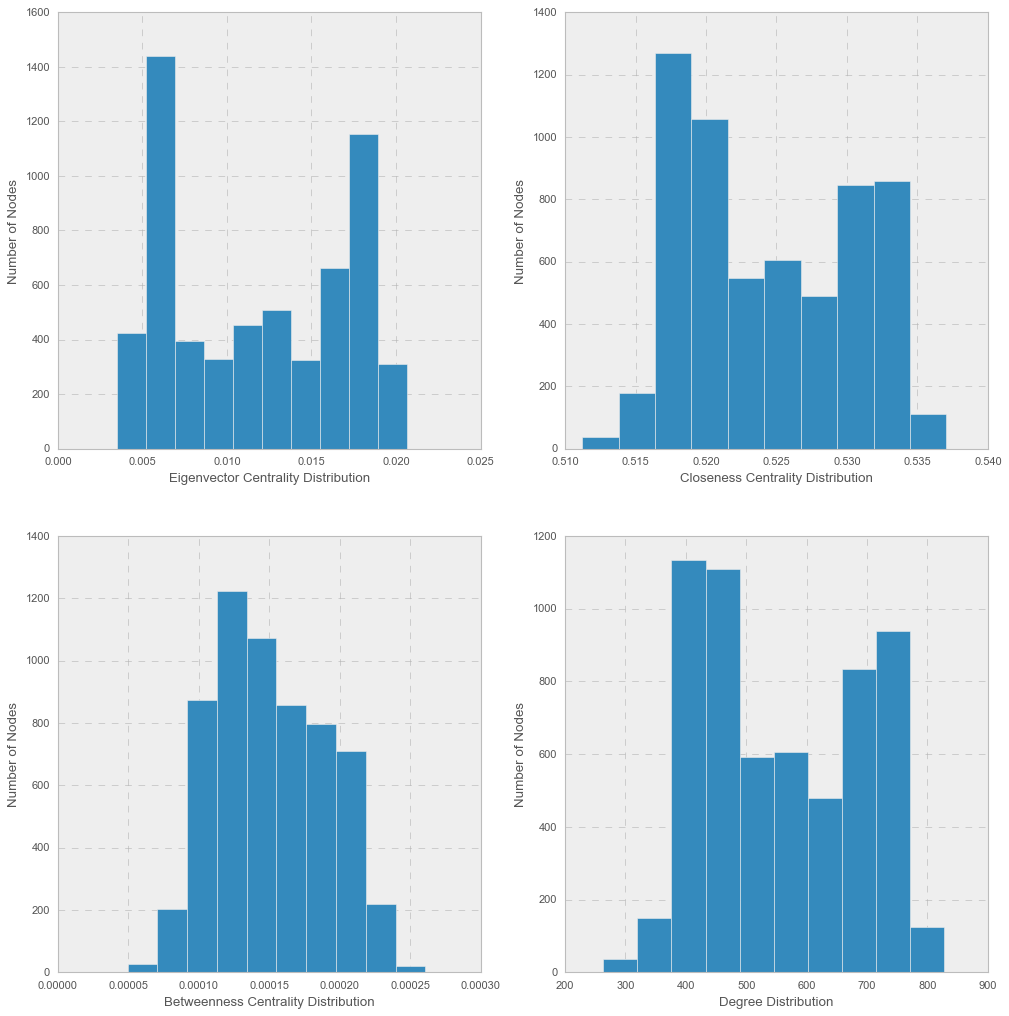
\includegraphics[width=0.7\textwidth]{centrality_measures.png}
	  \caption{Graph Statistics}
      \label{fig:centrality_measures}
  \end{figure}

  \noindent The network has a density of approximately 0.0933. This means that 
  9\% of the potential number of connections formed in the network.
  Nevertheless, when looking at the degree distribution histogram we can see, 
  that a all nodes have a large number of connections ranging between 263 -
  828 with an average of 559.63 connections. The distribution has two
  modes which likely correspond to the two main clusters shown in figure
  \ref{fig:us_airline_nodes}. The eigenvector centrality distribution shows, 
  that all nodes have a very low centrality measure and therefore none of the 
  nodes appear to have a large impact in terms of eigenvector centrality. The 
  closeness centrality distribution shows, that all nodes have an average 
  closeness centrality ranging from 0.51 - 0.53. This means that every node is 
  similarly connected and has an average impact for disseminating information 
  across the network. Lastly, the betweenness centrality distribution reveals 
  that there are no bottle-necks through which information flows. \\

  \noindent As a reference point, it is important to compare the properties of
  the created graph to real world graphs. For this thesis, the most appropriate
  networks for comparison are a social networks. Common structures of social 
  networks include \citep{watts1998collective,newman2006structure,Newman2010,
  kim2012multiplicative}:

  \begin{enumerate}
    \item Degree distributions often follow a power law distribution
    \item Emergence of a giant connected component
    \item Core-periphery structure
  \end{enumerate}

  \noindent The power law degree distribution and the emergence of a giant
  connected component creates network structures that have an onion
  (core-periphery) structure \citep[p. 121]{kim2012multiplicative}. This
  indicates, that most social networks have a few very highly connected nodes
  and many nodes with few connections. This creates a right skewed degree 
  distribution which also lead to a right skewed eigenvector centrality and
  closeness centrality distribution. For the betweenness centrality, it is 
  also expected, that more central nodes in a core-periphery network structure
  would exhibit some bottle-neck properties for the central nodes. For that
  reason one would expect central nodes to have a higher betweenness centrality.
  When looking at the distributions in figure \ref{fig:centrality_measures},
  this does not correspond to a power law degree distribution. The centrality 
  measures further do not correspond to the centralities frequently observed in 
  real social networks. The graph created with the MAG method does therefore 
  not share the properties observed in real social networks. In order to 
  generate a graph which shares the properties of real networks, one would have 
  to adapt the link-affinity properties to the core-periphery setting as shown 
  in figure \ref{fig:link-affinity}. This was tested and indeed an onion shaped
  network was created using the same attributes. Forcing this core-periphery 
  structure is however not purposeful for this thesis. Further, the aim of this 
  thesis is not necessarily to create realistic graphs rather than to create 
  useful graphs for graph machine learning. The results in chapter 
  \ref{section:results} reveal, that the graph is indeed useful for machine 
  learning. For that reason, the generated graph shown in this section is kept 
  for further analysis. 

  \subsection{Stochastic vs. Deterministic MAG}
  \label{section:stoch_det}

  As addressed in section \ref{section:self_survey}, the question was raised 
  as to whether the MAG should form connections between observations
  stochastically or whether a deterministic threshold probability yields better 
  results. The first insight gained when investigating this question lies in 
  the fact, that the probability of two observations is generally very low. 
  When setting the threshold probability for a connection between two 
  observations $u$ and $v$ to 0.5, not a single connection is made. This
  follows, as the probability for a connection decreases by design as the number 
  of attributes increases. This is implicitly shown in equation \ref{eq:MAG}, 
  where the product of probabilities is bound to decrease. For this reason, it 
  is suggested to limit the number of attributes to $K=\rho\log_{2}N$ for some 
  constant $\rho$ \citep[p. 122]{kim2012multiplicative}. The number of 
  attributes are selected accordingly such that $K\leqslant\log_{2} N$. The 
  US Airline Passenger dataset was used to generate a deterministic graph. The 
  threshold probability for a connection was set to 0.2 in the MAG model. The 
  MAG yielded several disconnected graphs which were for the most part 
  clustered according to their group memberships. Figure \ref{fig:det_MAG} 
  shows the graphs for the label and the attributes, where the edges are 
  removed. The subgraphs are unfortunately plotted very small, however all 
  subgraphs combined include all 6'000 nodes. The plots are meant to provide a 
  high-level overview of the generated subgraphs. 

  \begin{figure}[h]
		\centering
		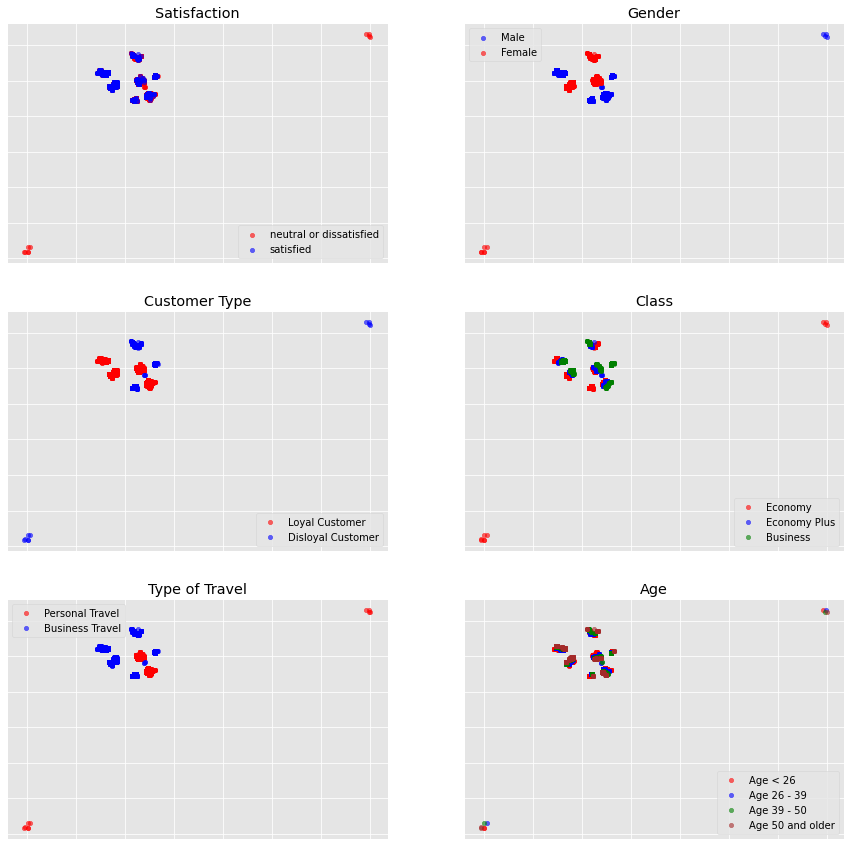
\includegraphics[width=1.0\textwidth]{deterministic_MAG.png}
		\caption{Deterministic MAG graph}
        \label{fig:det_MAG}
  \end{figure}

  \noindent The deterministic MAG model crates disconnected graphs which form 
  clusters based on node similarities. In terms of performance, the accuracy 
  and loss behavior of both the deterministic- and stochastic generated graphs 
  are virtually identical. This was true for all three datasets considered in 
  this thesis. For the purpose of visualization, stochastic graphs are more 
  useful, as one can identify the different cluster and their relationships to 
  one another on a single connected graph. For this reason, the stochastic graph 
  generation process is kept. Nevertheless, deterministic graph generation 
  appears to be useful if one wants to separate nodes in to more homogeneous 
  subgraphs. These subgraphs could then be used for subsequent machine learning 
  tasks with a cluster specific task in mind. The clusters further could 
  provide information as to which clusters tend to be more or less satisfied. 
  This is an area which could be interesting for future research.
  
